\chapter{Resultados}
\label{chap:resultados}

\drop{U}{na} vez adquiridos los conocimientos básicos sobre la estructura y funcionamiento del cerebro humano (sección \ref{sec::fisiologia}), así como sobre la neuroplasticidad\index{neuroplasticidad} (sección \ref{neuroplasticidad}) y el carácter maleable que ésta otorga al cerebro, en este capítulo se hace uso de esos conocimientos para la creación de un sistema de entrenamiento cerebral complejo. Además se ofrece una especificación detallada sobre cómo realizar una medición cuantitativa para poder valorar la evolución de dicho entrenamiento.

Por último se expondrán algunos algoritmos de recomendación que, haciendo uso de las métricas previamente definidas, permitirán encontrar usuarios afines a uno dado, así como juegos adecuados a un usuario en un instante concreto.

\section{Especificación del entrenamiento cerebral}
\label{sec:entrenamiento}
En base a la etapa de investigación documentada en las secciones \ref{sec::fisiologia} y \ref{neuroplasticidad}, las consideraciones que se han llevado a cabo para reconocer y diferenciar las capacidades mentales estimulables mediante el ejercicio agrupan estas capacidades en 5 grandes conjuntos:

\renewcommand{\labelenumi}{\bf\arabic{enumi}. }
\begin{enumerate}
\item Memoria
\item Resolución de problemas
\item Atención
\item Velocidad de procesamiento
\item Flexibilidad
\end{enumerate}

A continuación se presenta una jerarquía completa de las capacidades mentales consideradas, así como de las habilidades en que estas se han considerado subdivididas, detallándose el significado de cada una y cómo debe ser estimulada. En la figura \ref{fig::habilidades} se presenta un diagrama esquemático de dicha jerarquía.

\subsection{Memoria}

La mejora de la memoria se centra en tres aspectos realmente relevantes en la vida cotidiana: la memoria de trabajo, la memoria espacial y la memoria de asociación nombre-cara.

\begin{itemize}
\item {\bf Memoria de trabajo}

Procesos y estructuras de información empleados para el almacenamiento temporal y la manipulación de información durante el desarrollo de una tarea.

La memoria de trabajo requiere la activación de un circuito de neuronas, el cual activa en sí la memoria propiamente dicha. Esta memoria, si bien es activada desde la {\it corteza prefrontal}\index{córtex/corteza!prefrontal}, requiere a su vez la activación del resto de estructuras neuroanatómicas implicadas, como el \emph{lóbulo temporal}\index{lóbulo!temporal} para el significado o el \emph{lóbulo occipital}\index{lóbulo!occipital} para la imagen visual.

En un contexto informático, la memoria de trabajo se asemeja a la memoria RAM de un computador.

Los juegos para mejorar esta capacidad deben ofrecer pequeñas cantidades de información ---cada vez mayores según se aumente el nivel de dificultad--- durante un periodo corto de tiempo. El jugador debe asimilar esas porciones de información y recordarlas, para utilizarlas transcurrido un periodo de tiempo relativamente corto. El clásico juego de las parejas de cartas es un buen ejemplo. Otra posibilidad es ofrecer lecturas de párrafos cortos, y después jugar con esa información. Del mismo modo se puede jugar con otros sentidos, ofreciendo información auditiva, por ejemplo.

\item {\bf Memoria espacial}

Memoria responsable de registrar la información sobre el entorno y la orientación en el espacio.

Por ejemplo, en la vida real, la memoria espacial es la que nos permite recordar la ubicación del cuarto de baño de una casa ajena. De forma aún más sencilla, la memoria espacial nos permite trabajar en un escritorio, recordando dónde se encuentran los papeles, los lapiceros y bolígrafos, etc.

Los juegos dedicados al ejercicio y estimulación de esta capacidad mental deberán ofrecer un paisaje de objetos ---de complejidad variable, dependiendo de la dificultad de juego--- y dar un tiempo ---limitado o no--- para que el jugador memorice la localización de todos ellos. Después el jugador deberá reconstruir ese paisaje, de forma completa o parcial.

\item {\bf Memoria de asociación nombre-cara}

Se trata de los procesos relacionados con el registro y recuperación de la información que relaciona objetos visuales con objetos verbales. El caso más comprensible es el de la asociación entre las caras de las personas y sus nombres. Estimular esta capacidad incremente la habilidad para recordar el nombre de las personas que nos presentan y vemos por primera vez.

La estimulación de esta capacidad debe llevarse a cabo mediante el ejercicio de asociación de relacionar cada objeto de un conjunto con su único correspondiente de otro (u otros). Los juegos dedicados al trabajo de este tipo de memoria deberán mostrar la relación existente entre ciertos objetos y sus etiquetas, para permitir que el jugador pueda analizar y memorizar esas relaciones y reconstruirlas con posterioridad.

\end{itemize}

\subsection{Resolución de problemas}

Este conjunto se compone de las tres capacidades mentales que entran en juego a la hora de enfrentarnos y resolver cualquier tipo de problema: la aritmética, el razonamiento lógico y el razonamiento cuantitativo:

\begin{itemize}
\item {\bf Aritmética}

Esta capacidad mental consiste en la realización de operaciones matemáticas de forma correcta y rápida. Comprende la técnica de cálculo para las operaciones de suma, resta, multiplicación y división.

La estimulación de esta capacidad se llevará a cabo con la exposición del jugador a repetidas operaciones matemáticas sencillas. La resolución de muchas operaciones de pequeño tamaño obtiene mejores resultados que la resolución de pocas operaciones gigantescas.

\item {\bf Razonamiento lógico}

Es el proceso de lógica mediante el cual, partiendo de uno o más juicios, se deriva la validez o falsedad de otro juicio distinto. Tiene que ver con el reconocimiento de patrones y toma de decisiones.

Los juegos destinados a estimular esta habilidad consistirán en encontrar reglas ocultas clasificando objetos. Se mostrarán secuencialmente una serie de objetos, y el jugador debe indicar si cree que cada uno cumple o no una regla desconocida. A partir de sus aciertos y fallos deberá ir desentrañando la regla.

Por ejemplo, una partida puede consistir en la regla {\it ``polígonos con más de 4 lados y color rojo, verde o azul''}. El juego irá mostrando polígonos de diferentes colores y número de lados, y el jugador deberá indicar si cree que cada figura cumple o no la regla. Si una figura la cumple, el jugador sabrá que ese color y número de lados cumplen la regla, por lo que en un caso similar indicará que sí se cumple. Si la misma figura pero con un color diferente no cumple la regla, entonces el jugador aprenderá que el nuevo color no es aceptado por esa regla.

\item {\bf Razonamiento cuantitativo}

Como ya se dijo en la sección \ref{sec::problem-solving}, el razonamiento cuantitativo es utilizado por los seres humanos para realizar estimaciones.

Los juegos de razonamiento cuantitativo consistirán en la toma de decisiones simples en un corto espacio de tiempo. Dichas decisiones supondrán la elección de una opción entre varias, pudiendo ser el número mayor de entre un conjunto de números o resultados de operaciones, el lado que pesa más de una balanza con diferentes pesos a ambos lados, etc.

\begin{figure}[H]
  \begin{center}
    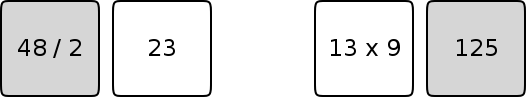
\includegraphics[width=0.5\textwidth]{./images/quantitative-reasoning.png}
    \caption{Decisiones de ejemplo para juegos de razonamiento cuantitativo: ¿Qué cuadrado de cada pareja tiene un valor mayor?}
  \end{center}  
\end{figure}

\end{itemize}

\subsection{Atención}

Este subconjunto de habilidades mentales se subdivide en 2 aspectos: Concentración y Campo visual.

\begin{itemize}

\item {\bf Concentración}

La concentración es la habilidad mental consistente en fijar los sentidos y pensamientos en una única tarea, objeto, etc. discriminando al resto. Es el filtrado de información sensorial, atendiendo una única fuente y discriminando el resto.

Los juegos de concentración consistirán en el enfrentamiento del jugador a una situación en la que tenga que centrarse en un único elemento de un conjunto homogéneo. Un posible juego de este tipo puede ser aquel que muestre una serie de objetos iguales apuntando en diferentes direcciones, obligando al jugador a indicar la dirección en la que apunta uno sólo de ellos. Cada grupo debe ser diferente, pero el objetivo debe seguir un patrón sencillo para que el usuario lo localice rápido y pueda indicar su respuesta. La figura \ref{fig::game-focus} muestra una posible aproximación, en la que los elementos son flechas y el jugador debe indicar dónde apunta la del medio.

\begin{figure}[h]
  \begin{center}
    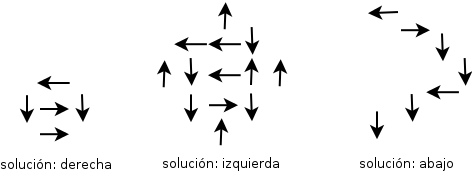
\includegraphics[width=0.8\textwidth]{./images/game-focus.png}
    \caption{Situación de ejemplo para un juego de concentración. El jugador indica (por ejemplo mediante las teclas de dirección), la dirección en la que el elemento central apunta.}
    \label{fig::game-focus}
  \end{center}  
\end{figure}

\item {\bf Campo visual}

El campo visual es el espacio que un individuo puede ver en un instante sin mover sus ojos. El diseño de juegos destinados a la estimulación de esta habilidad es sencillo: basta con mostrar varios elementos repartidos por el espacio de juego de forma simultánea, y luego, tras ocultarlos, solicitar al jugador que realice algún tipo de tarea con los objetos que se mostraron y ya no aparecen. Por ejemplo, se pueden mostrar varios números y, después de ocultarlos, pedirle al usuario que haga click en las ubicaciones aproximadas de los números por orden creciente o decreciente de valor.

\end{itemize}

\subsection{Velocidad de procesamiento}

Grupo mental centrado en la minimización del tiempo de respuesta ante estímulos y situaciones problemáticas. Se divide en las siguientes habilidades: Procesamiento de información y Orientación espacial:

\begin{itemize}

\item {\bf Procesamiento de información}

Habilidad consistente en la interpretación de la información sensorial. Tiene una relación directa con la capacidad de adaptación a los cambios del entorno.

Los juegos dedicados al entrenamiento del procesamiento de información consistirán en una serie de elementos mostrados secuencialmente, de uno en uno, de tal forma que algunos se repitan de forma consecutiva. Cuando el jugador ve cada elemento, indica si éste es exactamente igual que el anterior mostrado o no. Al responder se pasa al siguiente objeto, y así sucesivamente. El objetivo es responder de forma correcta el mayor número de veces en un tiempo limitado.

\item {\bf Orientación espacial}

La orientación espacial consiste en la consciencia tridimensional de la situación de un individuo en un entorno físico.

Los juegos dedicados a entrenar esta habilidad consistirán en un espacio bidimensional sobre el que se situarán elementos cuya posición memorizar. Después el mapa sufrirá algún tipo de transformación de {\it efecto espejo} o rotación, y el jugador tendrá que localizar dichas posiciones sobre el mapa modificado. Alternativamente, para el caso concreto de los juegos multijugador, otra posibilidad sería la de resolver un laberinto simétrico, empezando cada jugador por un extremo, y compitiendo por llegar antes que el otro al centro del laberinto. Dicho laberinto deberá sufrir transformaciones como las mencionadas, de tal manera que el desplazamiento por el mismo suponga la inversión de direcciones ---si el laberinto es rotado 90 grados en sentido horario, en el nuevo laberinto resultante las direcciones se verían alteradas: para desplazarse hacia arriba habría que usar la tecla izquierda, para moverse hacia la derecha habría que utilizar la tecla de dirección hacia arriba, y así sucesivamente---.

La figura \ref{fig::spatial-orientation} muestra un ejemplo de laberinto multijugador para un juego de estimulación de la orientación espacial.

\begin{figure}[h]
  \begin{center}
    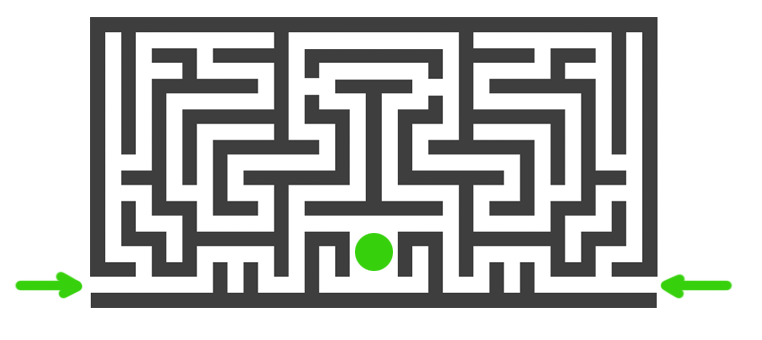
\includegraphics[width=0.8\textwidth]{./images/game-spatial-orientation.png}
    \caption{Escenario de ejemplo para un juego multijugador de orientación espacial}
    \label{fig::spatial-orientation}
  \end{center}  
\end{figure}


\end{itemize}

\subsection{Flexibilidad}

La flexibilidad es el subconjunto más amplio de habilidades mentales: {\it control de impulsos}, {\it planificación}, {\it conmutación de tareas} y {\it fluidez verbal} constituyen los aspectos relacionados con esta capacidad:

\begin{itemize}

\item {\bf Control de impulsos}

Como principal aspecto diferenciador entre el ser humano y el resto de animales, el control de impulsos permite priorizar unos objetivos por encima de posibles impulsos naturales.

Existen algunos juegos típicos relacionados con el control de impulsos que son muy buenos candidatos para ser implementados para BreakBrain. Son los juegos en los que se muestran palabras que representan a un color escritas en color (el mismo u otro). Por ejemplo se puede repetir de forma aleatoria, alternando los colores en los que las palabras aparecen escritas. El jugador debe indicar cuándo coincide el nombre del color representado por la palabra y el color en el que aparece.

\begin{figure}[h]
  \begin{center}
    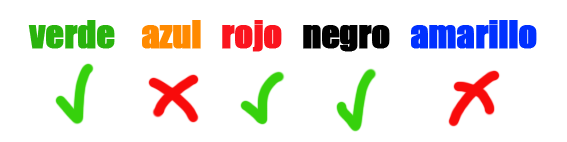
\includegraphics[width=0.6\textwidth]{./images/game-impulse.png}
    \caption{Ejemplo de prueba para ejercitar el control de impulsos}
  \end{center}  
\end{figure}

\item {\bf Planificación}

La planificación es la ordenación de tareas por prioridad a lo largo de un periodo temporal. Los juegos destinados a entrenar esta habilidad deben centrarse en la preparación de rutas sobre un escenario mediante pequeños cambios que vayan construyendo el camino. Esos cambios deben estar limitados en número o, alternativamente, utilizar los movimientos como penalización temporal para calcular la puntuación.

\item {\bf Conmutación de tareas}

La conmutación de tareas es la adaptación de la atención intercambiando entre diferentes ejercicios. Dependiendo de la situación (tarea actual) será conveniente actuar de una forma y no de otra.

Los juegos destinados a estimular y entrenar la habilidad de conmutación de tareas deben definir situaciones diferentes y asociar a cada una de ellas una forma de proceder. Una vez expuestas al jugador, dichas situaciones se alternarán de forma continuada, y el jugador tendrá que proceder como se espera en cada una de ellas. La figura \ref{fig::game-switch} muestra un ejemplo sencillo en el que varias flechas se desplazan en la misma dirección (diferente en cada actividad puntuable). Existen dos situaciones:

\begin{itemize}
\item Las flechas son rojas: el jugador debe indicar en qué dirección se mueven
\item Las flechas son verdes: el jugador debe indicar a qué dirección apuntan
\end{itemize}

Los dos escenarios se repiten, alternándose de forma aleatoria. El jugador debe responder, indicando la dirección que corresponda según la situación, en el menor tiempo posible.

\begin{figure}[h]
  \begin{center}
    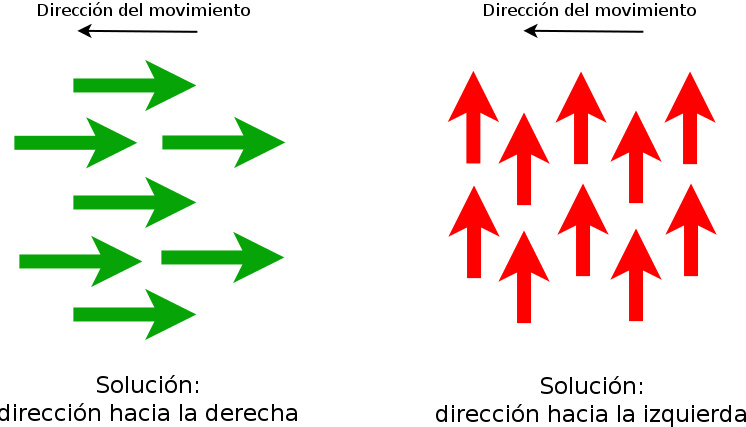
\includegraphics[width=0.6\textwidth]{./images/game-switch.png}
    \caption{Ejemplo de prueba para entrenar la conmutación de tareas}
    \label{fig::game-switch}
  \end{center}  
\end{figure}

\item {\bf Fluidez verbal}

Esta habilidad consiste en el acceso rápido al vocabulario conocido durante una tarea de escritura o una conversación. Resulta de vital importancia en la comunicación.

Los juegos dedicados a entrenar la fluidez verbal deben ofrecer partes de palabras (por ejemplo las dos o tres primeras letras) y permitir que el jugador vaya introduciendo palabras que cumplan ese patrón. Cada palabra correcta sumará una puntuación directamente proporcional a la longitud de la misma.

\end{itemize}


\begin{figure}[H]
  \begin{center}
    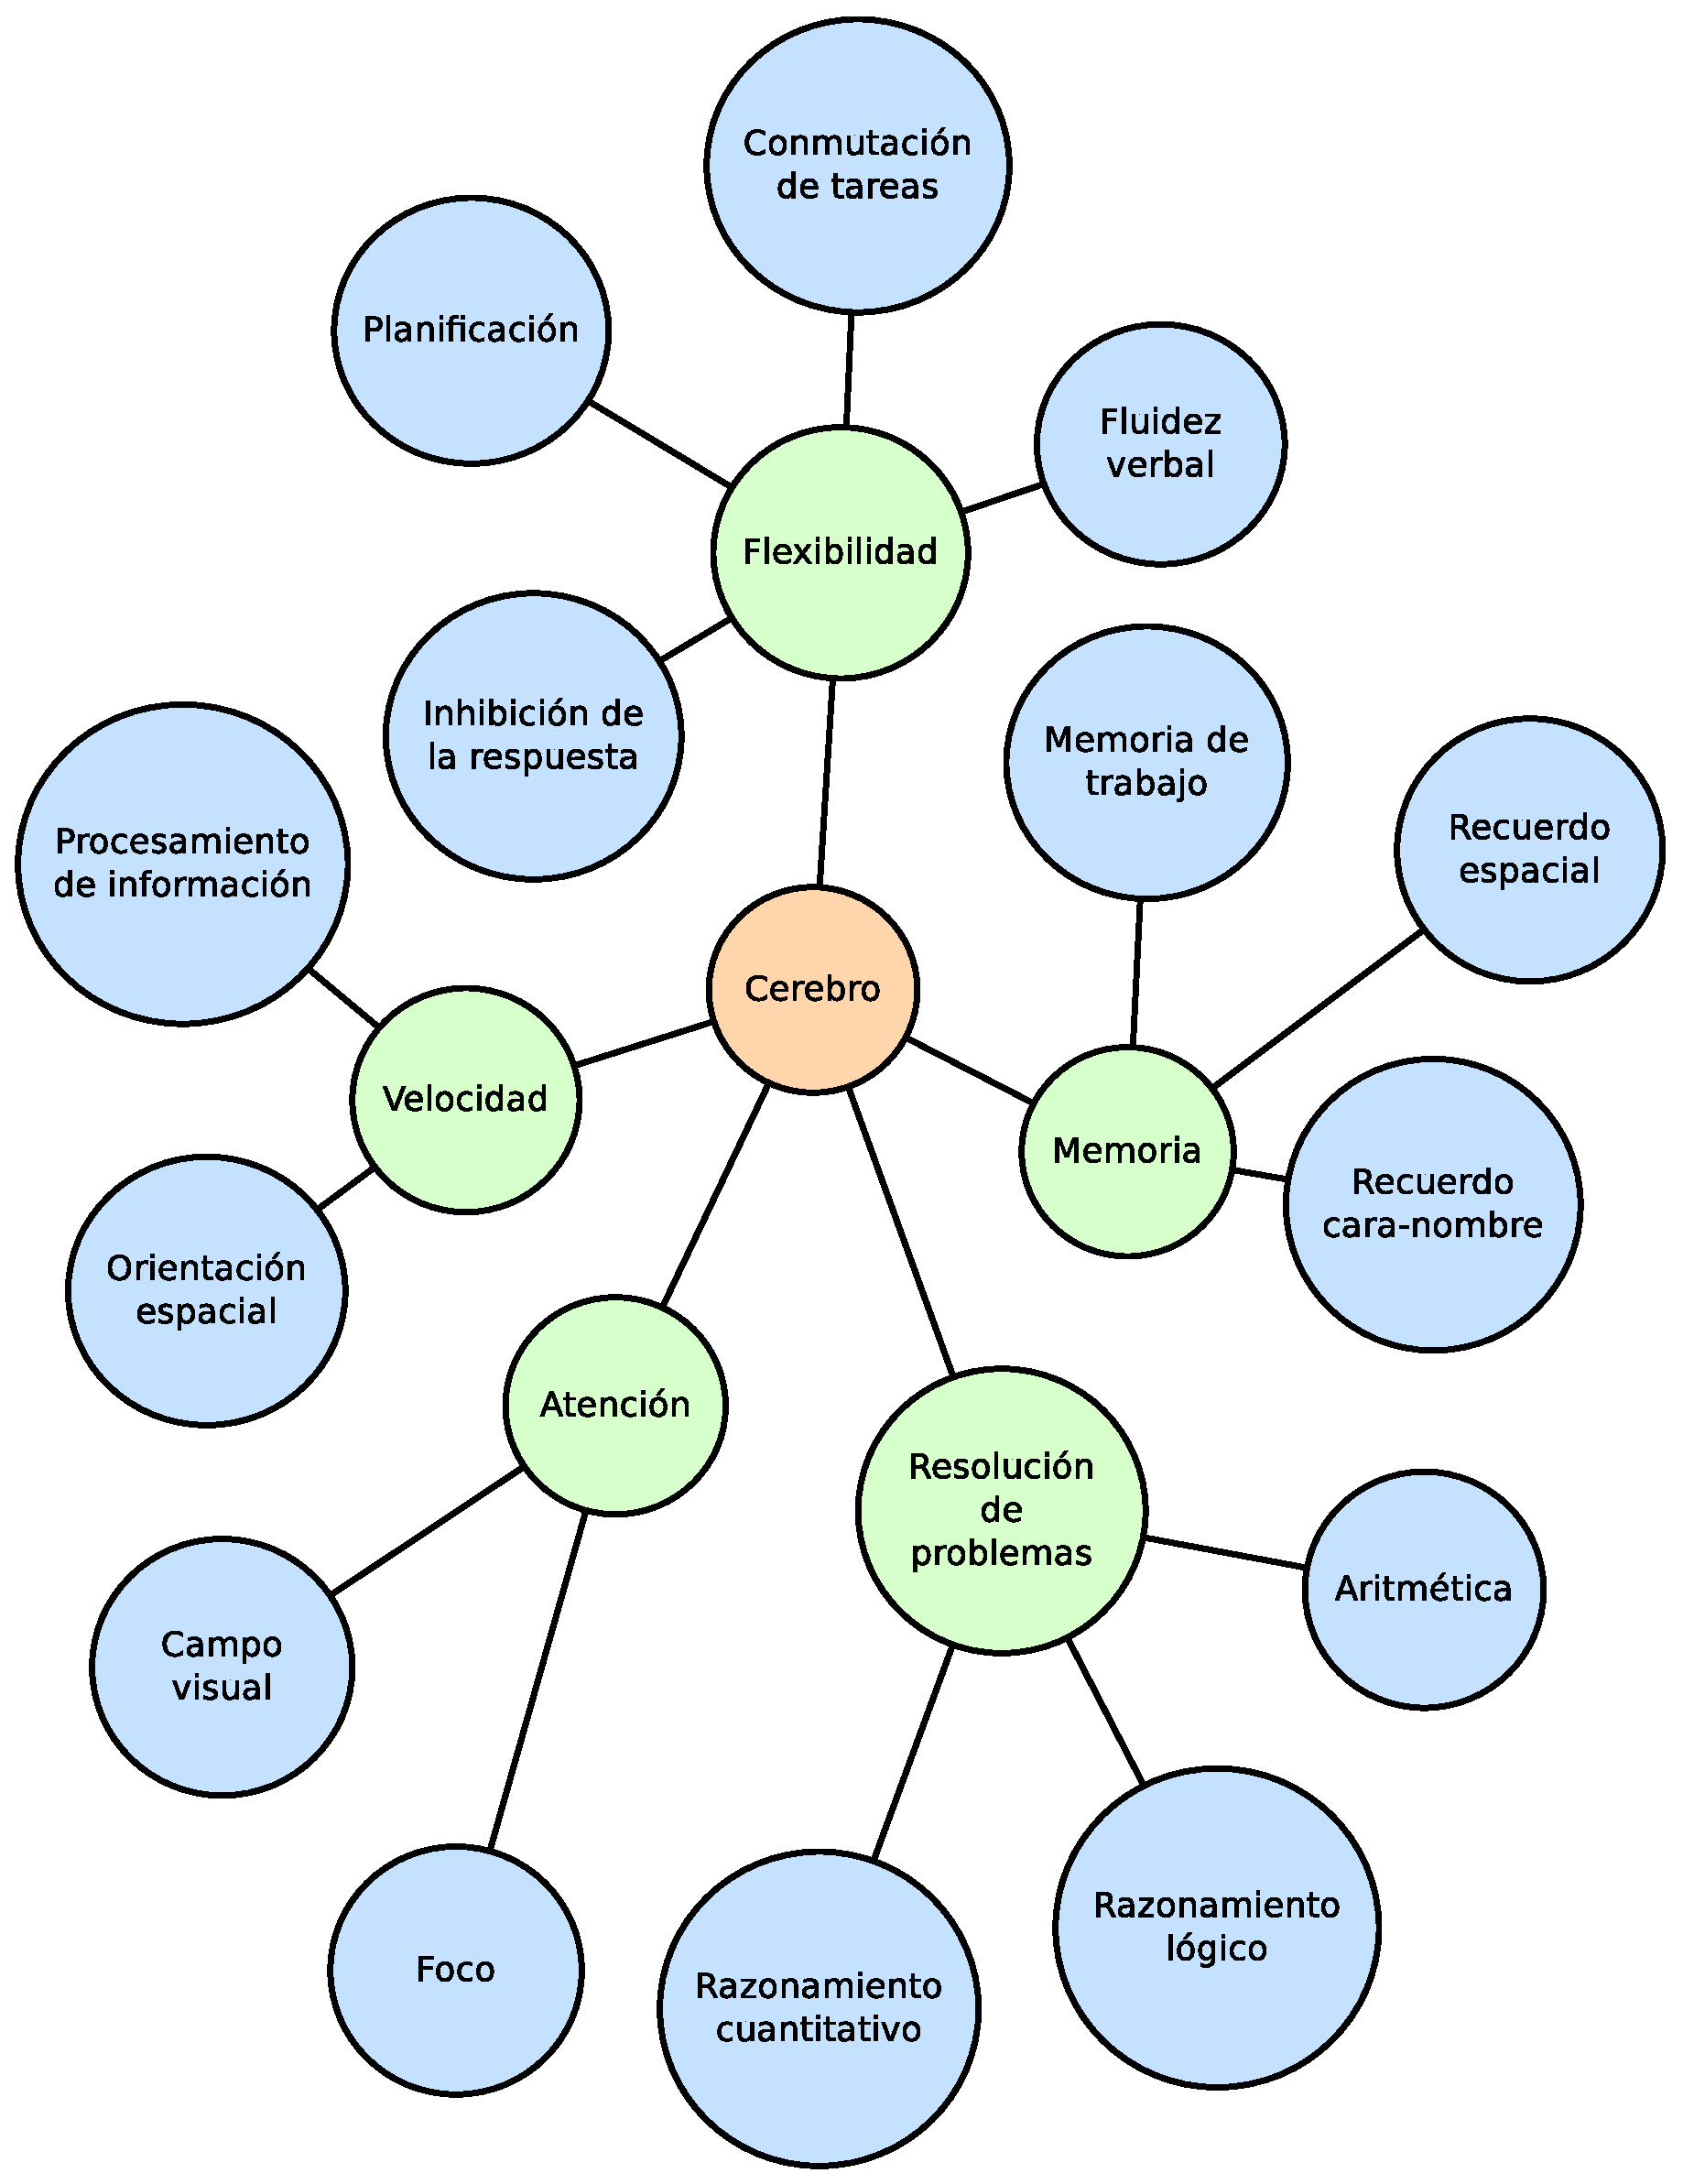
\includegraphics[scale=0.48]{images/games-diagram-esp.eps}
    \caption{Diagrama de capacidades y habilidades mentales}
    \label{fig::habilidades}
  \end{center}
\end{figure}


\section{Medición cuantitativa de la evolución cerebral}

A lo largo de esta sección se expondrán los conceptos básicos del diseño de la plataforma, para después desarrollar el sistema de puntuación de partidas y el conjunto de variables cerebrales que posibilitarán, por un lado la medición de la evolución de entrenamiento, y por otro la clasificación y recomendación de usuarios y juegos.

\subsection{Juegos, partidas y actividades puntuables}
\label{sec::juegos-partidas-actividades}

El diseño de BreakBrain hace distinción entre tres conceptos principales: juegos, actividades puntuables y partidas. En la figura \ref{fig::juegos-partidas-actividades} se ofrece una visión gráfica de la relación entre estos términos.

Resulta de vital importancia comprender bien estos conceptos para poder comprender el sistema de medición de la evolución de entrenamiento que ha sido creado en torno a ellos.

\subsubsection{Juego}

Un juego es una pequeña aplicación interactiva, centrada en una única habilidad mental (perteneciente a una capacidad), integrada en la plataforma y que permite su utilización por parte de uno o más usuarios de forma simultánea.

En base a la cantidad de jugadores que puedan enfrentarse entre sí en un juego, distinguimos entre juegos monojugador y juegos multijugador:

\begin{itemize}
\item {\bf Juegos monojugador}

Se trata de juegos diseñados para ser utilizados por un único usuario. No supone ningún tipo de interacción con otros usuarios. En este tipo de juegos no se gana o se pierde, sino que el resultado de los mismos es un valor cuantitativo que indica el grado de éxito de la partida (término que se estudia más adelante).

\item {\bf Juego multijugador}

En este caso se trata de juegos diseñados para ser utilizados por dos jugadores a la vez, suponiendo un enfrentamiento entre ellos. Sólo un jugador de los dos puede ganar cada ronda o partida (término que se estudia más adelante).

\end{itemize}

\subsubsection{Partida}

Una partida es cada una de las instancias jugables de un juego. Para ser más claros, cuando dos jugadores se encuentran jugando al mismo juego individual, cada uno en su máquina y sin realizar interacción alguna con el otro, cada uno de esos jugadores está jugando realmente una partida distinta del mismo juego.

Por otro lado, cuando dos jugadores se enfrentan cara a cara a un juego, compitiendo el uno contra el otro, ambos se encuentran en una misma partida de dicho juego. Obviamente en este caso siempre se tratará de juegos multijugador.

\subsubsection{Actividad puntuable}

La actividad puntuable es la unidad mínima jugable y, por lo tanto, la unidad mínima de entrenamiento y puntuación. Cada partida está compuesta por varias actividades puntuables. Por ejemplo, dado un juego de memoria en el que el usuario tiene que recordar la localización de grupos de objetos, cada actividad puntuable sería cada distribución de objetos a la que el usuario debe enfrentarse y resolver.

En base al número de actividades puntuables que las compongan, distinguimos entre los siguientes tipos de partidas:

\begin{itemize}
\item {\bf Partidas de corta duración}: Partida formada por 10 actividades puntuables
\item {\bf Partidas de duración media}: Partida formada por 30 actividades puntuables
\item {\bf Partidas de larga duración}: Partida formada por 50 actividades puntuables
\end{itemize}

\begin{figure}[H]
  \begin{center}
    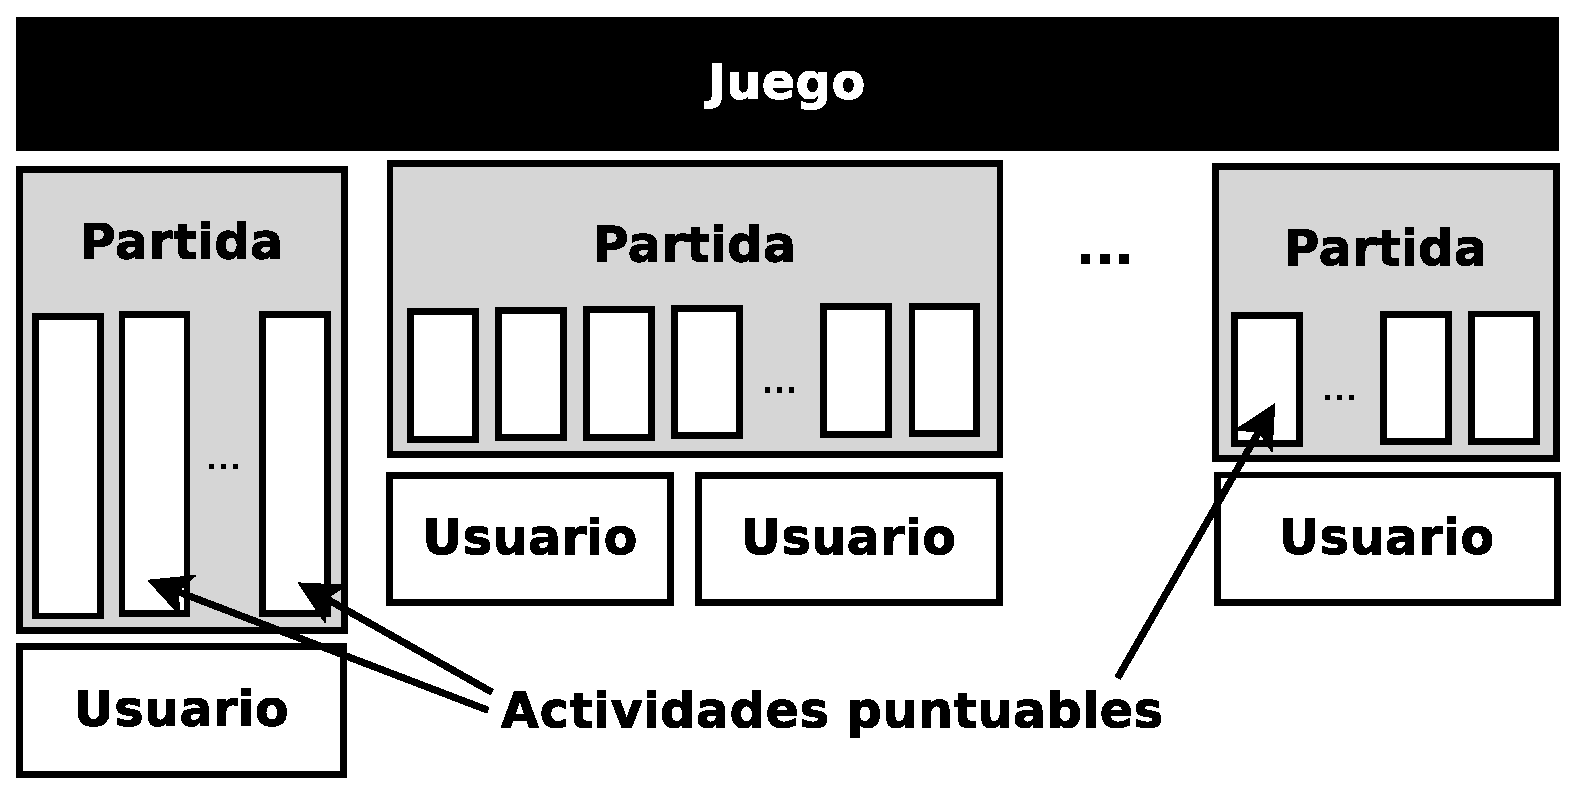
\includegraphics[width=0.8\textwidth]{images/juegos-partidas-actividades.eps}
    \caption{Juegos, partidas y actividades puntuables}
    \label{fig::juegos-partidas-actividades}
  \end{center}
\end{figure}

\subsection{Puntuación de partidas}

Tal y como se ha explicado en la sección \ref{sec::juegos-partidas-actividades}, una partida $p$ está compuesta por varias actividades puntuables $a_i$. La puntuación de una partida, $s_{p}$, es la suma de las puntuaciones obtenidas en cada actividad puntuable:


\begin{equation}
s_{p} = \sum\limits_{i = 0}^A s_i
\label{eq:partida}
\end{equation}

siendo $A$ el número total de actividades puntuables completadas en la partida $p$, y $s_i$ la puntuación de cada una de esas actividades.

La puntuación de cada actividad, $s_i$, se basa en dos aspectos: el tiempo empleado para completarla, $t_i$, y la valoración de éxito de la misma, $e_i$. Esta valoración de éxito puede ser satisfactoria o no satisfactoria, lo que matemáticamente se traduce en un 1 o un 0. Por otro lado, el tiempo $t_i$ debe encontrarse normalizado entre 0 y 1, para lo cual basta con dividir el tiempo empleado en realizar la actividad $i$ entre el tiempo empleado en realizar la actividad que más duración haya tenido. Teniendo en cuenta ambos aspectos, la puntuación de una actividad puntuable $a_i$ es la siguiente:

\begin{equation}
s_i = \frac{1}{t_i} \cdot e_i
\end{equation}

Reemplazando esta expresión en la ecuación \ref{eq:partida}, tenemos:

\begin{equation}
s_{p} = \sum\limits_{i = 0}^A \frac{1}{t_i} \cdot e_i
\end{equation}

Las actividades puntuables que no hayan sido completadas reciben una puntuación $s_i = 0$. Dependiendo del tipo de partida, será o no posible darla por finalizada sin haber completado todas las actividades puntuables que la constituyen:

\begin{itemize}
\item {\bf Puntuación en partidas monojugador}: el jugador recibe los puntos obtenidos en todas las actividades puntuables que constituyen la partida al finalizar la misma.
\item {\bf Puntuación en partidas multijugador}: una vez finalizadas todas las actividades puntuables de la partida por parte de uno de los jugadores, éste es considerado vencedor y la partida termina. Ambos jugadores reciben los puntos obtenidos durante la misma. En el caso del jugador perdedor, recibirá la puntuación de las actividades puntuables que haya completado satisfactoriamente antes de que el otro jugador haya terminado.
\end{itemize}

Teniendo en cuenta todo lo anterior, una partida $p$ formada por $A$ actividades puntuables tendrá una puntuación $s_p$ tal que $0 \leq s_p \leq A$.

\subsection{Variables de clasificación}

El perfil de cada usuario contiene la puntuación de cada habilidad cerebral, calculada mediante la suma de las puntuaciones obtenidas en cada partida de cada juego destinado a estimular esa habilidad. Además de ello contiene otras variables, como la cantidad de partidas ganadas, el sexo del individuo, etc. Todas estas variables se clasifican en 3 grupos:

\subsubsection{Variables estáticas o de agrupación}

\begin{itemize}
\item {\tt sex}: Sexo (hombre o mujer)
\item {\tt age}: Edad
\item {\tt keywords}: Palabras clave
\item {\tt training-interests}: Lista de habilidades mentales que el usuario está interesado en entrenar
\end{itemize}

\subsubsection{Variables dinámicas mentales}

\begin{itemize}
\item {\tt memory}: puntuación en el área de Memoria. Se trata de la suma de las siguientes tres puntuaciones:
  \begin{itemize}
  \item {\tt working-memory}: puntuación en memoria de trabajo.
  \item {\tt spatial-memory}: puntuación en memoria espacial
  \item {\tt face-name}: puntuación en memoria de asociación nombre-cara
  \end{itemize}
\item {\tt problem-solving}: puntuación en el área de Resolución de problemas. Se calcula mediante la suma de las siguientes tres puntuaciones:
  \begin{itemize}
  \item {\tt arithmetic}: puntuación en aritmética.
  \item {\tt logical-reasoning}: puntuación en razonamiento lógico.
  \item {\tt quantitative-reasoning}: puntuación en razonamiento cuantitativo.
  \end{itemize}
\item {\tt attention}: puntuación en la capacidad de Atención. Su valor es la suma de los valores de las siguientes dos variables:
  \begin{itemize}
  \item {\tt focus}: puntuación en la habilidad de concentración
  \item {\tt visual-field}: puntuación en campo visual
  \end{itemize}
\item {\tt speed}: puntuación en el área de Velocidad de procesamiento. Se trata de la suma de las siguientes dos variables:
  \begin{itemize}
  \item {\tt information-processing}: puntuación en procesamiento de la información
  \item {\tt spatial-orientation}: puntuación en orientación espacial
  \end{itemize}
\item {\tt flexibility}: puntuación en la capacidad de Flexibilidad. Se computa mediante la suma de las siguientes cuatro variables:
  \begin{itemize}
  \item {\tt response-inhibition}: puntuación en control de impulsos
  \item {\tt planning}: puntuación en planificación
  \item {\tt task-switching}: puntuación en conmutación de tareas
  \item {\tt verbal-fluency}: puntuación en fluidez verbal
  \end{itemize}
\end{itemize}

\subsubsection{Variables dinámicas sociales}

\begin{itemize}
\item {\tt followers}: cantidad de personas que siguen al usuario.
\item {\tt followees}: cantidad de personas a las que el usuario sigue.
\end{itemize}


\begin{table}[H]
\begin{footnotesize}
\label{table:capacidades}
\begin{center}  
\begin{sideways}
\begin{tabular}{|c|l|l|l|}
\hline
\tabheadformat
\tabhead{Grupo} & \tabhead{Habilidad} & \tabhead{Descripción} & \tabhead{Entrenamiento mediante juegos} \\
\hline\hline
\multirow{6}{*}{\begin{sideways}Memoria\end{sideways}} & Memoria  & Almacenamiento temporal de información & Mostrar pequeñas cantidades de información para memorizar \\
 & de trabajo & durante el desarrollo de una tarea. & y después requerirlas de algún modo. \\
\cline{2-4}
 & Memoria & Información del entorno, localización de objetos & Ofrecer un paisaje de objetos para su memorización \\
 & espacial & y orientación en el espacio. & y solicitar la reconstrucción del mismo.\\
\cline{2-4}
 & Memoria & Relación entre objetos y etiquetas asociadas & Mostrar la relación existente entre varios objetos y etiquetas.\\
 & nombre-cara & a dichos objetos.& El jugador deberá memorizar esas relaciones y reconstruirlas.\\
\hline\hline

\multirow{6}{*}{\begin{sideways}Res. prob.\end{sideways}} & Aritmética & Realización de operaciones matemáticas sencillas & Enfrentar al jugador a gran cantidad de operaciones sencillas.\\
\cline{2-4}
 & Razonamiento & Inducción de reglas lógicas & Mostrar elementos que cumplen o no una regla lógica para \\
 & lógico & a partir de casos concretos. & que el jugador la adivine y la aplique a otros elementos. \\
\cline{2-4}
 & Razonamiento & Realización de estimaciones y toma de decisiones & Ofrecer grupos de elementos cuantificables para que \\
 & cuantitativo & en base a ellas. & el jugador elija rápidamente el de mayor o menor valor. \\
\hline\hline

\multirow{4}{*}{\begin{sideways}Atención\end{sideways}} & Concentración & Fijación y dedicación de las actividades sensoriales & Ofrecer grupos de elementos en los que el jugador tenga que \\
 &  & a una única tarea. & prestar atención a alguna propiedad de uno sólo de ellos. \\
\cline{2-4}
 & Campo & Espacio tridimensional visible por un individuo sin & Mostrar y ocultar elementos en el espacio de juego. El jugador deberá \\
 & visual & realizar movimientos oculares. & realizar alguna tarea con las ubicaciones donde aparecían y su valor. \\
\hline\hline

\multirow{4}{*}{\begin{sideways}Velocidad\end{sideways}} & Procesamiento & Interpretación de la información sensorial. &  Ofrecer una secuencia de elementos, algunos idénticos consecutivamente. \\
 & de Información & Adaptación al cambio. & El jugador debe decir si cada uno es igual al anterior o no. \\
\cline{2-4}
 & Orientación & Consciencia tridimensional de la situación & Mostrar elementos distribuidos en un espacio. Tras una transformación \\
 & espacial & de uno mismo en el espacio. & del mismo, el jugador deberá localizar dichas posiciones. \\
\hline\hline
\multirow{8}{*}{\begin{sideways}Flexibilidad\end{sideways}} & Control de & Priorización de objetivos personales por & Jugar con los colores y su representación textual. El jugador \\
 & impulsos & encima de los impulsos animales. & deberá poder prestar atención a un sólo aspecto: el color o el texto. \\
\cline{2-4}
& Planificación & Priorización alterna de unas tareas sobre otras & Ofrecer un espacio bidimensional maleable mediante cambios. El jugador \\
& & en un periodo temporal. & construirá un camino usando el efecto de esos cambios. \\
\cline{2-4}
& Conmutación & Intercambio de la atención entre ejercicios de forma & Ofrecer situaciones diferentes, cada una con una misión. \\
& de tareas & arbitraria e intermitente. & Las situaciones van cambiando, y en cada una el jugador debe proceder. \\
\cline{2-4}
& Fluidez  & Recuperación rápida del vocabulario durante & Ofrecer las primeras o últimas letras de una palabra. El jugador \\
& verbal & una conversación fluida. & deberá enumerar palabras que cumplen ese patrón. \\
\hline
\end{tabular}
\end{sideways}
\end{center}
\end{footnotesize}
\caption{Ficha de entrenamiento de capacidades mentales}
\end{table}


% <<<<<<<<<<<<<<<<<<<<<<<<<<<<<<

\section{Sistema de recomendación}


\subsection{Algoritmo de recomendación de usuarios}

\subsection{Algoritmo de recomendación de juegos}

%% \subsection{Notas personales}

%% En \ref{sec::estructuras-primarias} se habla de la generación de patrones. Esto hay que comentarlo en los juegos.

%% En \ref{sec::corteza-cerebral} se habla de las áreas de Brodmann. Debería tenerlas en cuenta ne los juegos. La experiencia en la determinación de las representaciones corticales.

%% En \ref{sec::estructuras-subcorticales} se habla de como la experiencia afecta al cerebro

%\section{Algoritmo de búsqueda de usuarios}
